\chapter{Quantum Algorithms and Applications}
\label{chpt:algorithmsandapplications}

\epigraph{\textit{A quantum computation is like a symphony—many lines of tones interfering with one another}}{Seth Lloyd, Programming the Universe: A Quantum Computer Scientist Takes on the Cosmos}

% %\section{Introduction}
% \addcontentsline{toc}{section}{3.0 \hspace{0.3cm}Introduction}

\section{Introduction}\label{sec:algorithmsIntro}

In this chapter we review some of the well-known quantum algorithms that are thought to provide a speed-up over classical algorithms. This chapter should help to give the reader a sense of what future full scale quantum computer will be used for before continuing with more current short term applications in \autoref{chpt:shortqcomp}. In 1992, David Deutsch and Richard Jozsa proposed a quantum algorithm that is exponentially faster than any known deterministic classical algorithm \cite{deutsch1992}. Although the algorithm doesn't solve any problem of practical relevance, it was one of the first algorithms that demonstrated an exponential speed-up over classical algorithms. Soon after that, in 1994, Peter Shor proposed his famous factoring algorithm that sparked a huge interest in quantum computing and quantum cryptography \cite{shor1994}. A few years later in 1996, Lov Grover came up with an algorithm for the unstructured search problem which provides a quadratic speed-up over it's classical counterpart \cite{Grover1996}. Even though the speed-up for Grover's algorithm isn't exponential, it can be applied to a wide variety of problems including NP-complete problems. Since these algorithms were first proposed, a lot of research has been aimed at implementing them across a wide variety of different platforms. Even though quantum algorithms provide a speed-up over classical algorithms, it is worth noting that quantum algorithms are probabilistic in nature and may not always provide the correct answer. It is therefore necessary to evaluate the speed-up along with the probability of success when comparing quantum algorithms to their classical counterparts.

Most quantum algorithms exploit a unitary operation called the `oracle' operation. It is important to first understand the role the oracle operation plays in each algorithm and it therefore leads our discussion. We then go on to explain Deutsch-Jozsa's algorithm in \autoref{Deutsch-Jozsa}, included because of its historical importance as the first quantum algorithm. This is then followed by Grover's algorithm in \autoref{Grover-section}, presented as a useful example for developing some intuition about the probabilistic nature of quantum algorithms. It will also provide some insight into the use of superposition as a tool for quantum parallelism and amplitude amplification as a method for increasing the success probability of algorithms. In \autoref{Shor's algorithm} we give a brief introduction to Shor's algorithm, followed by quantum annealing in \autoref{sec:annealing} and the variational eigensolver algorithm in \autoref{sec:VQESolver}. The explanation of each algorithm is accompanied by examples to help make them more comprehensible and intuitive to understand. Finally, the algorithms, their resource requirements and success probabilities have been summarised in a table at the end of this chapter in \autoref{AlgorithmTable}.  

\section{The Oracle Operation}\label{Oraclular gates}

The oracle operation is used in each algorithm as a way of encoding the result of each computation into the quantum state which we can then extract through measurement. It should be thought of as a call to a function that we wish to learn about. It takes a state labelled $x$ and encodes the answer $f(x)$ into the resulting state. For example, suppose there is a function $f(x)$ on a one-bit domain range $x$ such that $f:\{0,1\}^n\mapsto\{0,1\}$. We can create a state $\ket{x,0}$ consisting of two registers, one for the domain $x$ and the other which we will use to store the answer $f(x)$ initially set to $0$. The oracle function would then encode the result of each bit string from the domain register into the range register. The operation transforms the state as follows:

\begin{equation*}
    \ket{x,0} \overset{O_{f}}{\longrightarrow} \ket{x,0 \, \oplus f(x)}
\end{equation*} 

where $\bigoplus$ indicates addition modulo 2. This is important since it will not always be the case that our range register is initialised to $0$ and in that case would be encoded via modulo 2 addition with $f(x)$, as seen in the next example. It is well known that this operation is unitary and can be simulated by an appropriate sequence of gates. This operation is usually referred to as the `bit oracle'. More importantly, if this operation is applied to the state $\ket{x,-}=\ket{x}(\ket{0}-\ket{1})/\sqrt{2}$, where the range resister is now initialised in the minus state $\ket{-}$ (see \autoref{twoQubit}) instead of the state $\ket{0}$, then the output state is given by:

\begin{equation*}
\begin{split}
  U_f\Big(\frac{1}{\sqrt{2}}\ket{x}\big(\ket{0}-\ket{1}\big)\Big) &=\frac{1}{\sqrt{2}}\ket{x}\big(\ket{0\oplus f(x)}-\ket{1\oplus f(x)}\big)\\
  &= (-1)^{f(x)}\frac{1}{\sqrt{2}}\ket{x}(\ket{0}-\ket{1}) 
\end{split}
\end{equation*}

This operation is a special case of the bit oracle and is generally known as the `phase oracle', denoted $U_{f}$ instead of $O_{f}$. It is an important part of many quantum algorithms as it allows the result of a computation to be encoded into the phase of a state which directly links the probability of each measurement outcome $x$ to its value $f(x)$. 


%%%%%%%%%%%%%%%%%%%%%%%%%%%%%%%%%%%%%%%%%%%%%%%%%%%%%%%%%%
\section{Deutsch-Jozsa algorithm}\label{Deutsch-Jozsa}
%%%%%%%%%%%%%%%%%%%%%%%%%%%%%%%%


The Deutsch-Jozsa algorithm is one of the first algorithms to demonstrate ``quantum parallelism''. In very simple terms, quantum parallelism is a feature of quantum computing which allows it to evaluate a function $f(x)$ simultaneously for many different values of $x$ via the use of superposition. Deutsch-Jozsa algorithm doesn't have many practical applications but it does provide insight into how quantum computing can trump classical computation. Suppose there is a function $f(x): \{0,1\}^{n} \rightarrow \{0,1\}$ which is either constant or balanced for all values of $x$, the Deutsch-Jozsa algorithm determines with certainty whether $f(x)$ is constant or balanced. A classical solver would need at least $N=2^{n}/2+1$ queries to determine with certainty whether the function is balanced or constant while the quantum algorithm can solve the problem in just one query. The box below describes how the Deutsch-Jozsa algorithm features the property of quantum parallelism for a 2-qubit case $(N=2^{2}=4)$. It should be noted that there is an additional qubit required for the implementation of the oracle which is not shown in the box below.

\begin{tcolorbox}[standard jigsaw,
    opacityback=0,  % this works only in combination with the key "standard jigsaw"
    boxrule=0.5pt,label={Deutsch's algorithm box}]
    {\bf Deutsch-Jozsa Algorithm}
    \tcbline
    \begin{enumerate}
    \item Start with the state $\ket{0}\ket{0}\ket{1}$.
    \item Apply Hadamard gate to all the qubits which leads to the state:\\
    \begin{center}
    $\ket{\Psi}=\dfrac{1}{2\sqrt{2}}\big(\ket{0}+\ket{1}\big)\big(\ket{0}+\ket{1}\big)\big(\ket{0}-\ket{1}\big)$.    
    \end{center}
    \item Apply the oracle `$U_{f}$' which transforms the state 
    $\ket{\Psi}$:\\
    \begin{center}
    $U_f\ket{\Psi}= \dfrac{1}{2\sqrt{2}}\big(\ket{0}-\ket{1}\big)\big[(-1)^{f(00)}\ket{00}+(-1)^{f(01)}\ket{01}+(-1)^{f(10)}\ket{10}+(-1)^{f(11)}\ket{11}\big]$
    \end{center}
    \item Apply the Hadamard to the first two qubits. If $f(x)$ is constant, the first two qubits end up in the state $\ket{00}$ but if $f(x)$ is balanced, the first two qubits are in the state $\ket{01}$, $\ket{10}$ or $\ket{11}$.
    \item Measuring the first two qubits reveals the nature of $f(x)$.
    \end{enumerate}
\end{tcolorbox}

The steps above can be extended to the $n$-qubit case and the circuit diagram for Deutsch-Jozsa algorithm for a general n-qubit case is given in \autoref{fig:deutsch}. Crucially the algorithm calls $f(x)$ once and evaluates it across the entire domain of $f$ at the same time. This is the power of superposition leading to inbuilt quantum computing parallelism. 
\begin{figure}[H]
\begin{equation*}
\Qcircuit @C=2.14em @R=1.25em
{\lstick{\ket{0}} & \gate{H} & \multigate{5}{U_f} & \gate{H} & \meter \\
\lstick{\ket{0}} & \gate{H} & \ghost{U_f} & \gate{H} & \meter \\ 
& \dot{} & & \dot{} \\
& \dot{} & & \dot{} \\
& \dot{} & & \dot{} \\
\lstick{\ket{0}} & \gate{H} & \ghost{U_f} & \gate{H} & \meter \\
\lstick{\ket{1}} & \gate{H} & \targ \qwx & \qw & \qw}
\end{equation*}
\caption{Circuit implementation of Deutsch-Jozsa algorithm for n-qubit input.}
\label{fig:deutsch}
\end{figure}

\begin{tcolorbox}[standard jigsaw,
    opacityback=0,  % this works only in combination with the key "standard jigsaw"
    boxrule=0.5pt,label={Deutsch's algorithm box}]
    {\bf Deutsch-Jozsa Algorithm (n-qubit case)}
    \tcbline
    \begin{enumerate}
    \item Start with the state $\ket{0}^{\otimes n}\ket{1}$, where $\ket{1}$ is the ancilla qubit required for the oracle.
    \item Apply the Hadamard gate to all the qubits in both registers.
    \item Apply the oracle `$U_{f}$' to the $n$ dimensional working register.
    \item Apply the Hadamard to the $n$ dimensional working register and measure them.
    \item If all the qubits are in the state $\ket{0}$, then the function $f(x)$ is constant, otherwise it is balanced.
    \end{enumerate}
\end{tcolorbox}
%%%%%%%%%%%%%%%%%%%%%%%%%%%%%%%%%%%%%%%%%%%%%%%%%%%%%




%%%%%%%%%%%%%%%%%%%%%%%%%%%%%%%
\section{Grover's algorithm} \label{Grover-section}
%%%%%%%%%%%%%%%%%%%%%%%%%%%%%%%


One of the earliest algorithms that was designed to use quantum resources is described in a 1996 paper by Lov Grover \cite{Grover1996}. The algorithm attempts to solve the following problem: imagine you have a database of elements. We can represent them as bit strings but we know that one of them is `marked' by some function acting on that bit string. Examining the case where we have 4 numbers (2 bits), suppose we have the following truth table with the third element as marked. 

\begin{equation}
\begin{array}{c|c|c}
    & x & f(x) \\
    \hline
    0 & 00 & 0 \\
    1 & 01 & 0 \\
    2 & 10 & 1 \\
    3 & 11 & 0 \\
\end{array}
\end{equation}

This unstructured search is an important problem in computer science. If we used a classical computer to try to find the marked element `10' above we'd have to call $f(x)$ at most 3 times, since it could always end up being the last element applied to $f(x)$. The number of attempts scales as expected, with order $N$, $O(N)$. Specifically, it takes at most $N$ attempts to find the marked element out off N possible elements.

However, using the principle of superposition, we can explore the whole space of elements simultaneously. To do this we need two gates. The first one  flips the phase of the marked element leaving all other the same. For the marked element being '10' as above, we have

\begin{equation}
U_f = \begin{blockarray}{cccc}
    \ket{\textcolor{blue}{00}} & \ket{\textcolor{blue}{01}} & \ket{\textcolor{red}{10}} & \ket{\textcolor{blue}{11}} \\
    \begin{block}{(cccc)}
        1 & 0 & 0 & 0\\
        0 & 1 & 0 & 0\\
        0 & 0 & -1 & 0\\
        0 & 0 & 0 & 1\\
    \end{block}
\end{blockarray}
\end{equation}

The second ingredient is the following matrix, (irrespective of which element is marked).

\begin{align}
        D = \frac{1}{2}\begin{pmatrix}
        -1 & 1 & 1 & 1 \\
                 1 & -1 & 1 & 1\\
                 1  & 1 & -1 & 1 \\
                 1 & 1 & 1 & -1
        \end{pmatrix}
\end{align}

Now we will look at the algorithm step-by-step for this simple four element (two qubit) case. Starting with the qubits in the `00` state, we generate a superposition using a so called Hadamard gate (represented by H) on each qubit, which takes $\ket{00} \rightarrow \ket{00} + \ket{01} + \ket{10} + \ket{11}$ (we have ignored normalisation for simplicity). This can be represented by the matrix transformation:

\begin{align}
        H \otimes H \ket{00} = 
        \frac{1}{2}
        \begin{pmatrix}
        1 & 1 & 1 & 1 \\
        1 & -1 & 1 & -1\\
        1  & 1 & -1 & -1 \\
        1 & -1 & -1 & 1
        \end{pmatrix}
        \begin{pmatrix}
        1\\
        0\\
        0\\
        0\\
        \end{pmatrix}
        =
        \frac{1}{2}
        \begin{pmatrix}
        1\\
        1\\
        1\\
        1\\
        \end{pmatrix}
        = \frac{1}{2}(\ket{00} + \ket{01} +\ket{10} + \ket{11})
\end{align}

In the next step of the algorithm, we apply the phase oracle $U_f$ (see \autoref{Oraclular gates}). This picks out the marked element, giving it a minus sign. This $U_f$ gate is in fact exactly the phase oracle previously described:

\begin{align}
    U_f \ket{x}=(-1)^{f(x)}\ket{x},  
    f(x) = \begin{cases}
        1 & \text{if x is marked}  \\
        0 & \text{if x is unmarked} \\
    \end{cases}
\end{align}

Applying this gate gives:

\begin{align}
        U_f\frac{1}{2}(\ket{00} + \ket{01} +\ket{10} + \ket{11})
        =\frac{1}{2}
        \begin{pmatrix}
        1 & 0 & 0 & 0 \\
        0 & 1 & 0 & 0\\
        0  & 0 & -1 & 0 \\
        0 & 0 & 0 & 1
        \end{pmatrix}
        \begin{pmatrix}
        1\\
        1\\
        1\\
        1\\
        \end{pmatrix}
        =
        \frac{1}{2}
        \begin{pmatrix}
        1\\
        1\\
        -1\\
        1\\
        \end{pmatrix}
        =\frac{1}{2}(\ket{00} + \ket{01} - \ket{10} + \ket{11})
\end{align}

The final step is to apply $D$. The application of gate $D$ can be understood as an operation which increases the amplitude of the phase shifted element in the previous step, suppressing the amplitude of the others. This can be thought of as a constructive interference on the marked element and destructive interference on all of the other elements. 

\begin{align}        
    \frac{1}{2} D (\ket{00} + \ket{01} - \ket{10} + \ket{11})
    =\frac{1}{2}.\frac{1}{2}
    \begin{pmatrix}
    -1 & 1 & 1 & 1\\
    1 & -1 & 1 & 1 \\
    1 & 1 & -1 & 1 \\
    1 & 1 & 1 & -1 \\
    \end{pmatrix}
    \begin{pmatrix}
    1 \\ 1 \\ -1 \\ 1 
    \end{pmatrix}
    =
    \frac{1}{4}
    \begin{pmatrix}
    0 \\ 0 \\ 4 \\ 0
    \end{pmatrix}
    = 
    \begin{pmatrix}
    0 \\ 0 \\ 1 \\ 0
    \end{pmatrix}
    =\ket{10}
\end{align}

From this we can see that the general recipe of Grover's algorithm is to create a superposition of all the possible states, add a $\pi$ phase shift to the marked states with the special unitary $U_f$, and then use $D$ to pick out this phase shift.

In this case the algorithm has successfully found the marked element with certainty (though this does not take into account any experimental imperfections observed in real life). However, using superposition inevitably leads to success with a non-unity success rate, as demonstrated in the next section, where we look at the three qubit case described using Dirac notation instead of matrices, as now we would have to use $2^3 \times 2^3$ matrices. Hence the transition to Dirac notation is a natural progression for larger system sizes. 

%%%%%%%%%%%%%%%%%%%%%%%%%%%%%%%%%%%%%%%%%
\subsubsection{Three qubit case}
Here we consider the problem on $N=8$ elements, where the fifth element is marked. Crucially, this change to a larger number of qubits means that the problem is no longer solved with certainty. The algorithm can be applied with a minimum of $3$  ($2^{3}=8$) qubits in the following manner. Here we have let the marked element be the 5th element '100':

\begin{tcolorbox}[standard jigsaw,
    opacityback=0,  % this works only in combination with the key "standard jigsaw"
    boxrule=0.5pt,label={example100100000}]
    {\bf Grover's Algorithm on three qubits}
    \tcbline
    \begin{enumerate}
    \item Start with the state $\ket{000}$.
    \item Apply the Hadamard gates which result in the state: $\ket{\Psi}=\dfrac{1}{2\sqrt{2}}\big(\ket{000}+\ket{001}+\ket{010}+\ket{011}+\ket{100}+\ket{101}+\ket{110}+\ket{111}\big)$
    \item Apply $U_{f}$, which reverses the sign (adds a $\pi$ phase shift) on the fifth element: $\ket{\Psi}=\dfrac{1}{2\sqrt{2}}\big(\ket{000}+\ket{001}+\ket{010}+\ket{011}-\ket{100}+\ket{101}+\ket{110}+\ket{111}\big)$
    \item Apply D, which leads to state $\ket{\Psi}=\dfrac{1}{4\sqrt{2}}\big(\ket{000}+\ket{001}+\ket{010}+\ket{011}+5\ket{100}+\ket{101}+\ket{110}+\ket{111}\big)$
    \item Repeat steps 3 and 4 ``$T$'' times, where $T$ is to be determined later.
    \item Measure the state $\ket{\Psi}$.
    \end{enumerate}
\end{tcolorbox}



\begin{figure}
    \centering
    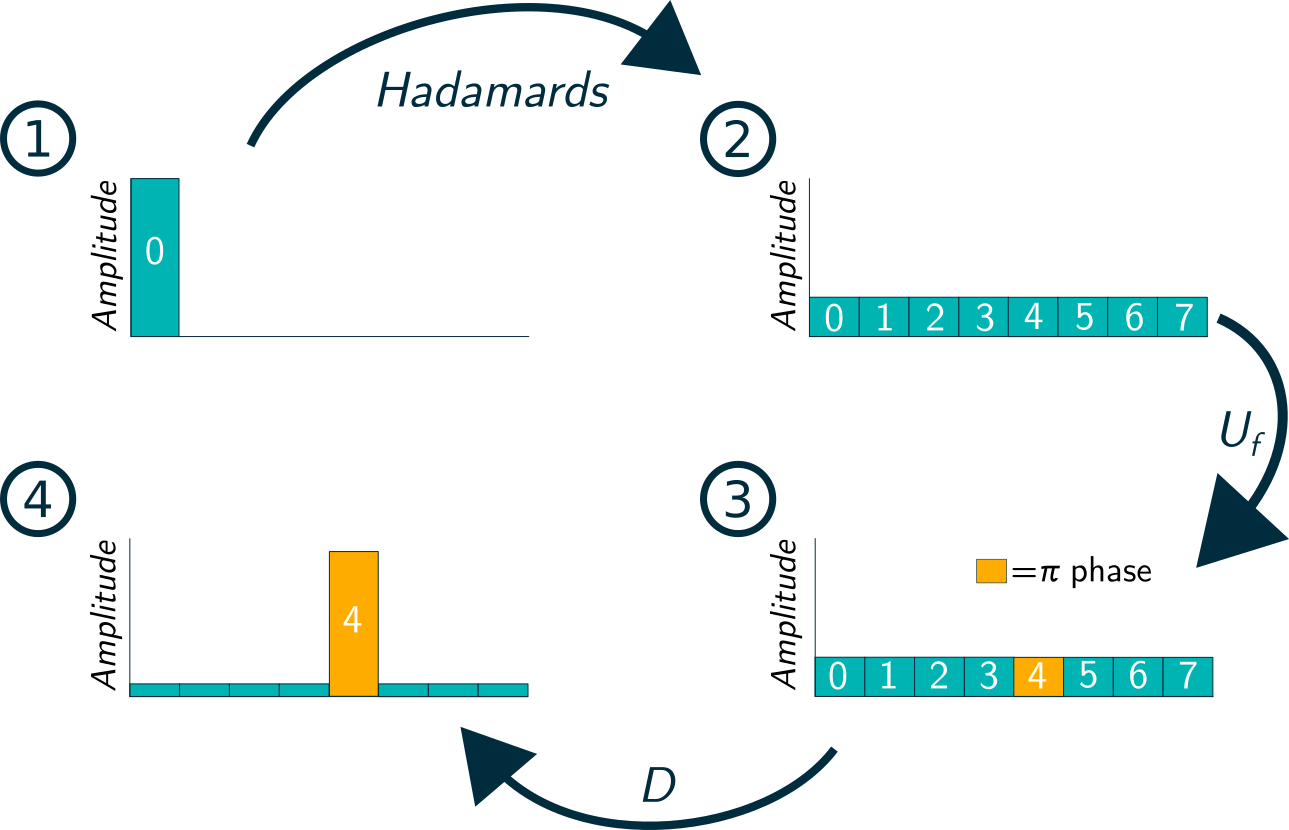
\includegraphics[width=0.9\linewidth]{figures/Grovers.png}
    \caption{Pictorial demonstration of the steps of Grover's Algorithm}
    \label{fig:Grovers}
\end{figure}



Whereas for two qubits applying the combination of $U_fD$ once was sufficient to find the marked element with certainty, with more qubits we must be careful about the number of times this combination is applied. Repeating these two gates on the state gives an oscillating probability for finding the correct element. For clarification, if we carry out another iteration of steps 3 and 4 in the above example, we get the state:
\begin{align}
\ket{\Psi}=\dfrac{-1}{8\sqrt{2}}\big(\ket{000}+\ket{001}+\ket{010}+\ket{011}-11\ket{100}+\ket{101}+\ket{110}+\ket{111}\big).
\end{align}
 Now if a measurement is performed on this state, there is a 94.5\% chance of getting the fifth element compared to 78.1\% probability after just one iteration. If yet another iteration of step 3 and 4 is performed, the resulting state becomes:

\begin{align}
\ket{\Psi}=\dfrac{-7}{16\sqrt{2}}\big(\ket{000}+\ket{001}+\ket{010}+\ket{011}-\frac{13}{7}\ket{100}+\ket{101}+\ket{110}+\ket{111}\big)    
\end{align}
and the probability of getting the marked element upon measurement decreases again to 67\%. Therefore, it is important to choose the number of iterations for Grover's algorithm carefully. The number of iterations ``$T$'' required to get the maximum probability of measuring the marked element is approximately given by:

\begin{equation}\label{groverIteration}
    T \approx \frac{\pi}{4}\sqrt{N} - \frac{1}{2}
%    T=\big(\pi\big/4)\sqrt{N}
\end{equation}


%%%%%%%%%%%%%%%%%%%%%%%%%%%%%%%%%%%%
\subsubsection{General n-qubit case}

Given a function $f: \left\{0,1\right\}^n \rightarrow \left\{0,1\right\}$ with the promise that $f(x_0) = 1$ for a unique element $x_0$, the problem is to find this $x_0$. We use a quantum circuit on $n$ qubits in the initial state $\ket{0}^{\otimes n}$.

\begin{tcolorbox}[standard jigsaw,
    opacityback=0,  % this works only in combination with the key "standard jigsaw"
    boxrule=0.5pt,label={example100100000}]
    {\bf Grover's Algorithm on n-qubits}
    \tcbline
    \begin{enumerate}
    \item Start with the state $\ket{0}^{\otimes n}$.
    \item Apply the Hadamard gates to each qubit result in the state: $\ket{\Psi}=\dfrac{1}{\sqrt{n}}\sum_{x\in\{0,1\}^n}\ket{x}$
    \item Apply $U_f\ket{x} = (-1)^{f(x)}\ket{x}$, which reverses the sign of the marked element.
    \item Apply D where $D = -H^{\otimes n}U_0H^{\otimes n}$.
    \item Repeat steps 3 and 4 T times, where $T=\frac{\pi}{4}\sqrt{N} - \frac{1}{2}$.
    \item Measure the state $\ket{\Psi}$.
    \end{enumerate}
\end{tcolorbox}

The circuit implementation of Grover's algorithm is given in \autoref{fig:grovercircuit}.\\

\begin{figure}[H]
\begin{equation*}
\Qcircuit @C=2.14em @R=1.25em
{\lstick{\ket{0}} & \gate{H} & \multigate{5}{U_f} & \multigate{5}{D} & \multigate{5}{U_f} & \ghost{U_f} & \lstick{\dots} & \multigate{5}{D} & \meter \\
\lstick{\ket{0}} & \gate{H} & \ghost{U_f} & \ghost{D} & \ghost{U_f} & \ghost{U_f} &\lstick{\dots} & \ghost{D} & \meter \\ 
& \dot{} & & & & & & & \dot{} \\
& \dot{} & & & & & & & \dot{} \\
& \dot{} & & & & & & & \dot{} \\
\lstick{\ket{0}} & \gate{H} & \ghost{U_f} & \ghost{D} & \ghost{U_f} & \ghost{U_f} & \lstick{\dots} & \ghost{D} & \meter \\}
\end{equation*}
\caption{Circuit implementation of Grover's algorithm.}
\label{fig:grovercircuit}
\end{figure}

\subsubsection{Construction of gate $D$ and $U_{f}$}
The gate $D$ in Grover's algorithm applied on $n$-qubits can be can be decomposed into smaller gates as shown in \autoref{fig:gateD}. This shows that gate $D$ requires $2n+1$ Hadamard ($H$) gates, $2n+1$ Pauli $X$ gates and an n-control Toffoli gate.

\begin{figure}[H]
\begin{align*}
\Qcircuit @C=1.14em @R=1.25em
{\lstick{\ket{x_1}} & \gate{H} & \gate{X} &  \ctrl{1} & \gate{X} & \gate{H} & \qw  \\
\lstick{\ket{x_2}} & \gate{H} & \gate{X} &  \ctrl{4} & \gate{X} & \gate{H} & \qw  \\
\lstick{\dot{}} & \dot{} & \dot{} & & \dot{} & \dot{} & \\
\lstick{\dot{}} & \dot{} & \dot{} & & \dot{} & \dot{} & \\
\lstick{\dot{}} & \dot{} & \dot{} & & \dot{} & \dot{} & \\
\lstick{\ket{x_n}} & \gate{H} & \gate{X} &  \ctrl{1} & \gate{X} & \gate{H} & \qw  \\
\lstick{\ket{0}} & \gate{X} & \gate{H} &  \targ & \qw & \qw & \qw }
\end{align*}
\caption{Decomposition of gate '$D$' into Hadamard, Pauli X and n-control Toffoli gates.}
\label{fig:gateD}
\end{figure}

The construction of gate $U_{f}$ is not as straight forward as for the D gate above and in general is dependent on which algorithm being used. We have coded the oracle function required for Grover's algorithm in several languages in \autoref{chpt:implementations}. 

%%%%%%%%%%%%%%%%%%%%%%%%%%%%%
\section{Shor's algorithm}

\label{Shor's algorithm}

Shor's algorithm describes a procedure for factorising large numbers. Given an $n$-digit integer $N$, Shor's algorithm determines whether $N$ is prime and in the case it is not, the algorithm outputs a non-trivial factor of $N$. The algorithm consists of mainly classical ingredients with one computationally heavy step outsourced to a quantum computer. The first part of Shor's algorithm consists of a classical algorithm that determines the greatest common divisor (gcd) of two integers. This is efficiently achieved by using Euclid's algorithm. The second part of the algorithm involves finding the periodicity of a discrete periodic function. This is achieved by employing a period finding algorithm and it is this step that utilises a quantum algorithm. The box below describes the Shor's algorithm in more detail. 

\begin{tcolorbox}[standard jigsaw,
    opacityback=0,  % this works only in combination with the key "standard jigsaw"
    boxrule=0.5pt,label={Shor's algorithm box}]
    {\bf Shor's algorithm for factorising N}
    \tcbline
    \begin{enumerate}
    \item Check if N is even, if so output 2. Else, Pick an initial guess $a<N$.
    \item Calculate the greatest common divisor of $a$ and $N$, gcd($a,N$). If we obtain a number other than 1, then we have found a factor of $N$, so output gcd$(a,n)$ as our factor for $N$.
    \item Otherwise, find the period of the function $f(x) = a^x \mod N$. Label this period $r$. If we found $r$ to be odd then this method has failed: return to step 1. 
    \item Since  $a^0 \mod N = a^r \mod N = 1$, then $a^r - 1 \mod N = 0$. Factoring, $a^r-1 \mod N = (a^{r/2} - 1)(a^{r/2} + 1) \mod N = 0$. Thus $(a^{r/2} - 1)(a^{r/2} + 1) = lN$ for some integer $l$. 
    \item Output either gcd($a^{r/2}-1$) or gcd($a^{r/2}+1$) as the factors of $N$.
    \end{enumerate}
\end{tcolorbox}

Currently no efficient classical algorithm is known to solve step 3. However, using a quantum algorithm the problem can be solved exponentially faster than the best known classical algorithms. We shall now explain the machinery behind this process, aimed more at developing an intuition for the quantum effects rather than the fine detail of the process.

\autoref{fig:ShorCircuit} shows a circuit to implement Shor algorithm. The $1^{st}$ register is acted upon by Hadamard gates to put the qubits in a uniform superposiiton. The second step uses the bit oracle operation $O_f$ for the periodic function $f(x)=a^x \mod N$ which has the following effect on the second registers:

\begin{equation}
    U_{a^x \mathrm{mod} N}\ket{x}\ket{0}= \ket{x}\ket{a^x \mathrm{mod} N}
\end{equation}


\begin{figure}
    \centering
    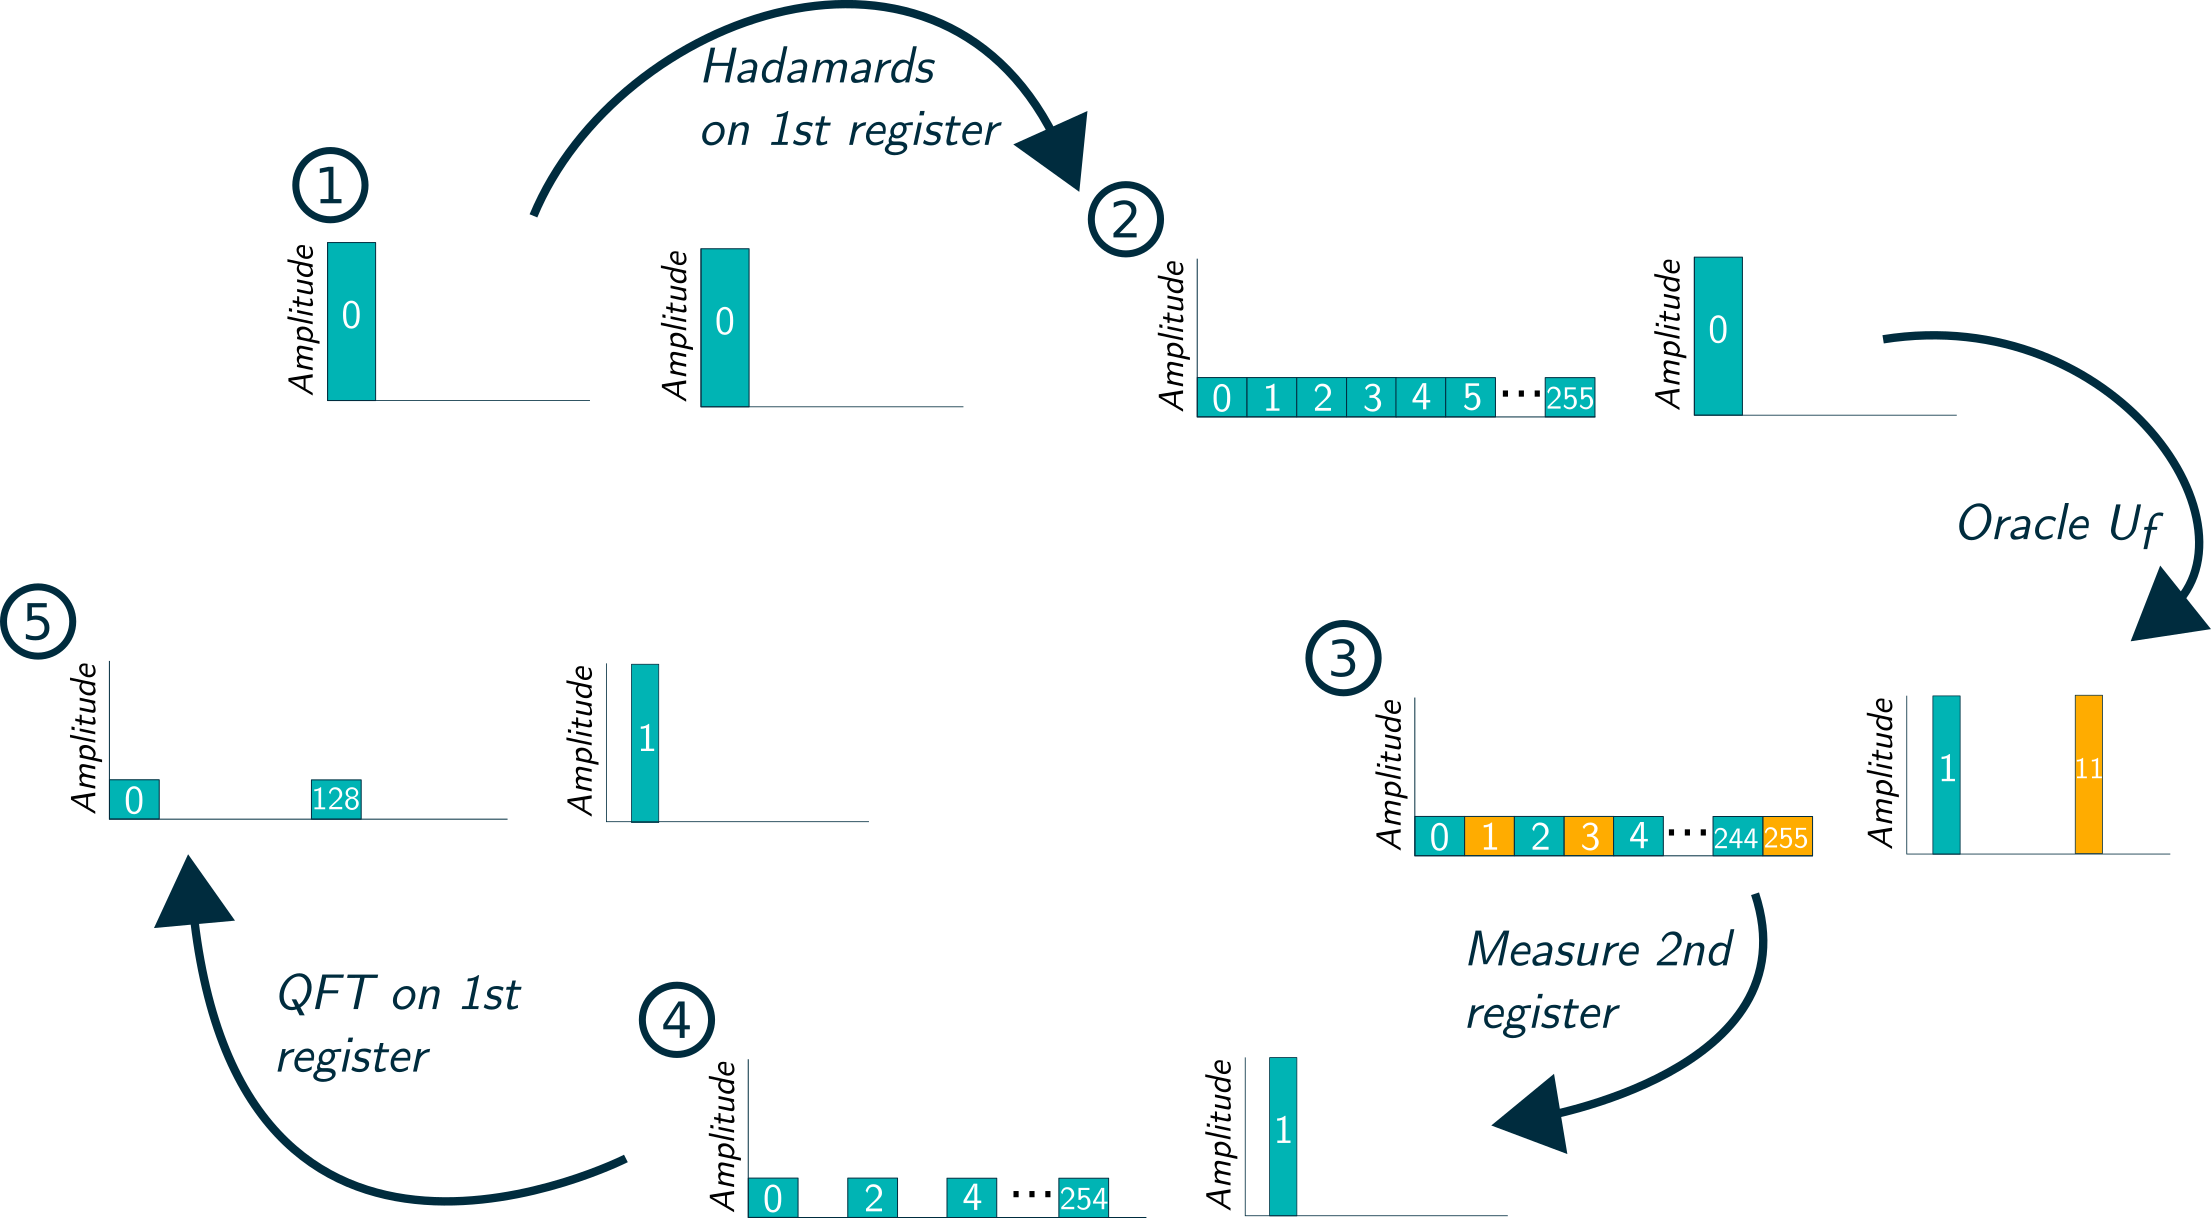
\includegraphics[width=\linewidth]{figures/Shors.png}
    \caption{Diagram of the quantum aspects of Shor's algorithm to factor 15, using $a=11$. In step 3, the different colours show which qubit values in the 1st and 2nd registers are associated to each other, a demonstration of entanglement. When the first register is measured, there is a 50\% chance of success - if 128 is measured and divided by $2^8=256$, we can extract the correct value of $r=2$ from the resulting fraction $l/r = 1/2$}
    \label{fig:Shors}
\end{figure}

Measuring the second register then collapses the state to basis states equal to $f_0 = f(x_0)$, where $f(x_0) = f(x_0 + r) = f(x_0 + 2r) = ...$ where $r$ is the periodicity of the function. Thus the first register is now in a superposition of the states $\ket{x_0+jr}$ for all integers $j$ allowed for $x_0+jr$ to be within the register. Therefore we have a periodic superposition of states, generating peaks in the probability distribution of measurement outcomes that correspond to the values $x_0$, $x_0+r$, $x_0+2r$... as can be seen in step 4 of \autoref{fig:Shors}. We can then extract the period with the quantum fourier transform.

\subsection{Quantum Fourier Transform}

One of the most useful transformations in mathematics is the discrete Fourier transform. The quantum Fourier transform (QFT) is exactly the same transformation apart from the fact that QFT is applied to quantum states. For example the QFT acting on two qubits is given by the transformation matrix:

\begin{align}
    QFT = 
    \frac{1}{2}
    \begin{pmatrix}
        \omega_N^{0} & \omega_N^{0} & \omega_N^0 &\omega_N^0 \\
        \omega_N^0 & \omega_N^1 & \omega_N^2 & \omega_N^3 \\
        \omega_N^0 & \omega_N^2 & \omega_N^4 & \omega_N^6 \\
        \omega_N^0 & \omega_N^3 & \omega_N^6 & \omega_N^9 \\
    \end{pmatrix}
    =
    \frac{1}{2}
    \begin{pmatrix}
        1 & 1 & 1 & 1 \\
        1 & i & -1 & -i \\
        1 & -1 & 1 & -1 \\
        1 & i & -1 & i \\
    \end{pmatrix}
\end{align}

This can be generalised to $n$ qubits, which requires a $2^n$ dimensional matrix with elements given by 

\begin{align}
    QFT_{jk} \equiv \omega_N^{jk} = \exp^{2\pi ijk / N} 
\end{align}

where we the columns and rows of the matrix are indexed from 0. The Quantum Fourier Transform can be constructed out of more fundamental quantum gates, a Hadamard gate and a controlled phase gate. 

 \begin{align}
    H = 
    \begin{pmatrix}
    1 & 1 \\
    1 & -1 \\
    \end{pmatrix},
    \quad
    R_k = 
    \begin{pmatrix}
    1 & 0\\
    0 & \omega_{2^k}\\
    \end{pmatrix}
 \end{align}
 
 This requires $n(n-1)/2$ controlled phase gates in total and $n$ Hadamard gates. 

The circuit diagram given by \autoref{fig:qft} shows how QFT is implemented on an $n$-qubit state $\ket{x_1 \ldots x_n}$ using Hadamard and controlled phase gates. The QFT outputs a state in the form $\ket{y_n \ldots x_1}$ and swap gates are used at the end of QFT to correct the order of the output state.


\begin{figure}
\begin{align*}
\Qcircuit @C=1.0em @R=1.55em
{\lstick{\ket{x_1}} & \gate{H} & \gate{R_2} & \qw & \lstick{\dots} & \lstick{\dots} & \gate{R_{n-1}} & \gate{R_n} & \qw & \qw & \qw & \qw & \qw & \qw & \qw & \qw &\qw & \qw & \qw & \qw & \qw & \qw & \rstick{\ket{y_n}}\\
\lstick{\ket{x_2}} & \qw & \ctrl{-1} & \qw & \lstick{\dots} & \lstick{\dots} & \qw & \qw & \gate{H} & \qw & \lstick{\dots} & \lstick{\dots} & \gate{R_{n-2}} & \gate{R_{n-1}} & \qw & \lstick{\dots} & \lstick{\dots} & \qw & \qw & \qw & \qw & \qw & \rstick{\ket{y_{n-1}}}\\
%\lstick{\dot{}} & & \dot{} & & & & \\
\lstick{\vdots} & & \vdots & & & & \\ \\
%\lstick{\dot{}} & & \dot{} & & & & \\
\lstick{\ket{x_{n-1}}} & \qw & \qw & \qw & \qw & \qw & \ctrl{-4} & \qw & \qw & \qw & \qw & \qw & \ctrl{-3} & \qw & \qw & \lstick{\dots} & \lstick{\dots} & \gate{H} & \gate{R_2} & \qw & \qw & \qw & \rstick{\ket{y_2}}\\
\lstick{\ket{x_{n}}} & \qw & \qw & \qw & \qw & \qw & \qw & \ctrl{-5} & \qw & \qw & \qw & \qw & \qw & \ctrl{-4} & \qw & \lstick{\dots} & \lstick{\dots} & \qw & \ctrl{-1} & \qw & \gate{H} & \qw & \rstick{\ket{y_1}}}
\end{align*}
    \caption{Efficient circuit for the quantum Fourier transform.}
    \label{fig:qft}
\end{figure}


\begin{figure}
\begin{align*}
\Qcircuit @C=2.14em @R=1.8em
{
& & & \lstick{\ket{0}} & \gate{H} & \multigate{7}{O_f} & \qw & \multigate{4}{QFT} & \meter \\
& & &\lstick{\vdots} & \vdots &                         &              &         & \lstick{\vdots}  \\
& \push{\mathrm{1^{st}\,register}} & &\lstick{\ket{0}} & \gate{H} &           \ghost{O_f} & \qw &\ghost{QFT} & \meter \\
&   &&\lstick{\ket{0}} & \gate{H} &           \ghost{O_f} & \qw &\ghost{QFT} & \meter \\
&                   &&\lstick{\ket{0}} & \gate{H} &           \ghost{O_f} & \qw &\ghost{QFT} & \meter \\
&                   &&\lstick{\ket{0}} & \qw &               \ghost{O_f} &  \meter \\
& \push{\mathrm{2^{nd}\,register}}              & &\lstick{\vdots} &       &                   &\lstick{\vdots} \\
&                   &&\lstick{\ket{0}} & \qw &       \ghost{O_f} & \meter  \gategroup{1}{3}{5}{3}{1.7em}{\{}
\gategroup{6}{3}{8}{3}{1.7em}{\{}}
\end{align*}
\caption{Circuit implementation of Shor's algorithm.}
\label{fig:ShorCircuit}
\end{figure}

%%%%%%%%%%%%%%%%%%%%%%%%%%%
\section{Quantum annealing}
\label{sec:annealing}
%%%%%%%%%%%%%%%%%%%%%%%%%%%

Quantum annealers are a type of optimisation algorithm. They  can directly solve Quadratic unconstrained binary optimization (QUBO) problems. Given the coefficients $Q_{ij}$, the QUBO problem is to determine the minimum value of

\begin{equation}
C=\sum_{i=1}^{N} Q_{ii}x_i+\sum_{i<j}^{N} Q_{ij}x_ix_j\\\\\ x_i\in\{0,1\}.
\end{equation}

This type of problem is essential in the application ranging from graph theory \cite{lucas_2014} to machine learning \cite{ogorman_2015},\cite{adachi_henderson}.\\

To give a better idea of what is QUBO problem, we will use the example of the light switching game taken from \href{https://www.dwavesys.com/tutorials/background-reading-series/quantum-computing-primer}{D-Wave's quantum computing primer} \cite{dwave}. Imagine there are several lights with certain bias marked for each of them and certain weights assigned between every two of them. For each switch, "ON" scores 1 point and "OFF" scores 0 point. The total score is the sum of the bias multiplied by the light configuration score. Furthermore, there is an additional score contribution if adjacent lights are both on. The goal is to set the light configuration such that the total score is minimised. If we have a positive bias for all of the lights and connections, it is intuitive to see such a configuration is setting all the light to "OFF". However, it is notoriously complicating to take the weights between the lights into account as well.Here is where the quantum annealer comes about.\\


% \subsection{Boolean logic}
% It is interesting to address that Boolean logic can be written as QUBO form
% %%%%%%%%%%%%%%%%%
% \begin{table}[h!]
% \centering
% \begin{tabular}{|l|l|}
% \hline
% Boolean logic     & Corresponding QUBO                   \\ \hline
% $x_1= NOT x_0$    & $-x_0-x_1+2x_0x_1$                   \\ \hline
% $ x_2=x_0 OR x_1$ & $x_0+x_1+x_2+x_0x_1-2x_0x_1-2x_0x_2$ \\ \hline
% $x_2=x_0 AND x_1$ & $3x_2+x_0x_1-2x_0x_2-2x_1x_2$        \\ \hline
% \end{tabular}
% \caption{Boolean logic in QUBO form}
% \end{table}

%%%%%%%%%%%%%%%%%%%%%
\subsection{Coloring}

 One of the NP problems which can be implemented in QUBO form is the vertex coloring problem.
 Given the graph G(V, E) with the set of vertices V and the set of edges E, the problem is to determine the coloring configuration of the vertices for which no adjacent two nodes (the nodes connected with edge) have the same color. \\ 
Mathematically it is the same as finding the minimum value for:

\begin{equation}\label{graphProblem}
H = \sum_{n=0}^{N-1}(1-\sum_{k=0}^{K-1}x_{n,k})^2 + \sum_{(u,v)\in E}\sum_{k=0}^{K-1}x_{u,k}x_{v,k}
\end{equation}

$x_{n,k}$ with node $n$ and color $k$ is $1$ only if the node $n$ has color $k$ and $0$ otherwise. $N$ is the total number of nodes and $K$ is total number of colors used. The first term is the restriction that each node can only have one color. The second term is the restriction that the adjacent nodes have different color. As only one dimensional QUBO problems can be solved by current quantum annealers, Equation \ref{graphProblem} must be reduced to a one dimension problem by reordering the index $n,k \rightarrow nK+k$.
This results in
\begin{equation}
H = \sum_{n=0}^{N-1}(1-\sum_{k=0}^{K-1}x_{nK+k})^2 + \sum_{(u,v)\in E}\sum_{k=0}^{K-1}x_{uK+k}x_{vK+k}
\end{equation}
Further expansion and reduction using $x_i^2=x_i$ gives
\begin{equation}
H= \sum_{n=0}^{N-1}(1+\sum_{k_1=0}^{K-1}\sum_{k_2=0}^{K-1}x_{nK+k_1}x_{nK+k_2}-\sum_{k=0}^{K-1}x_{nK+k})+ \sum_{(u,v)\in E}\sum_{k=0}^{K-1}x_{uK+k}x_{vK+k}
\end{equation}
This can be input directly into D-Wave system.

%%%%%%%%%%%%%%%%%%%%%%%%%%%%%%%%%%%%%%%
\section{Variational Quantum Eigensolver (VQE) Algorithm}\label{sec:VQESolver}
%%%%%%%%%%%%%%%%%%%%%%%%%%%%%%%%%%%%%%%

\addcontentsline{toc}{subsection}{4.2.0 \hspace{0.3cm}Introduction}

%We have already listed some NISQ algorithms, particularly optimisation algorithms. The VQE algorithm is an instance of the QAOA algorithm. The idea here is the following. 

The dynamics of physical systems (examples materials and molecules) is modelled by Hamiltonians which are represented by Hermitian (self-adjoint) matrices. The modelling of these hamiltonians is important for the material science and developments of new drugs which involves working with huge of these Hermitian matrices representing complex molecules. Observables associated to these molecules, particularly the Energy of the system, and furthermore, the ground state energy of the system. So the problem here is an eigenvalue problem, given a (potentially huge) Hermitian matrix, finding the lowest eigenvalue. We can do this classically, but for huge matrices it requires a lot of resource (example here), so here is where the VQE offers speed ups REF.

\begin{tcolorbox}[standard jigsaw,
    opacityback=0,  % this works only in combination with the key "standard jigsaw"
    boxrule=0.5pt,label={VQEbox}]
    {\bf The problem:}
    \tcbline
    Given a physical system (say a molecule) represented by a $n$-qubit Hamiltonian $H$. The matrix $H$ is an Hermitian matrix and therefore by the Spectral decomposition theorem it can be diagonalised in terms of its eigenvalues $\{\lambda_i\}$ eigenvectors $\{\ket{\lambda_i}\}$ as:
    \begin{align}H=\sum^n_{i=0} \lambda_i \ket{\lambda_i} \bra{\lambda_i},
    \end{align}
    These eigenvectors form a basis. without loss of generality we can order the eigenvalues in increasing order $\lambda_0<\lambda_1<...<\lambda_n$, so that the lowest eigenvalue $\lambda_0$ and associated eigenvector$\ket{\lambda_0}$ and $H \ket{\lambda_0}=\lambda_0 \ket{\lambda_0}$. These eigenvalue and eigenvector are also called ground energy and ground state. We are interested in finding the lowest eigenvalue. 
\end{tcolorbox}


\begin{tcolorbox}[standard jigsaw,
    opacityback=0,  % this works only in combination with the key "standard jigsaw"
    boxrule=0.5pt,label={VQEbox}]
    {\bf Classical Solution: Eigenvalue problem}
    \tcbline
    Classically, and by virtue of the spectral decomposition theorem, the diagonalisation of $H$ can, in principle, always be done, but here the question is if it can be done \emph{efficiently}.
\end{tcolorbox}

%%%%%%%%%%%%%%%
\begin{comment}
By virtue of $\lambda_0$ being defined as the ground energy we have that
\begin{align*}
    \left< \lambda_0|H| \lambda_0\right>=\lambda_0 \leq \lambda_i= \left<\lambda_i|H| \lambda_i\right> \hspace{0.5cm} \forall i \neq 0
\end{align*}
\end{comment}
%%%%%%%%%%%%%

%%%%%%%%%%%%%%%
%%%%%%%%%%%%%%%
\begin{comment}
We have access to a quantum device capable of implementing $n$-qubit states. We take the state of the system to the ansatz state $\ket{\psi(\theta)}$. We then can apply gates so that we can implement $H$ as a gate, so we then have the state $H\ket{\psi(\theta)}$. After this, we can measure the system in a base containing the ansatz state $\ket{\psi(\theta)}$, and therefore we can obtain the expected value for the energy of the system when in state $\ket{\psi(\theta)}$ which is given by  $\lambda_{\psi(\theta)}:=\left< \psi(\theta)|H| \psi(\theta)\right>$. This expected value is always greater or equal than the ground energy (See aside for a derivation):
\begin{align}
\lambda_{\psi(\theta)} \geq \lambda_0, \hspace{0.5cm}\forall \ket{\psi(\theta)},
\label{eq:inequality}
\end{align}
 With the help of a classical minimisation optimiser to move over the parameter(s) $\theta$ and after sampling enough times one should expect to be considerable close to the ground energy $\lambda_0$, and therefore the algorithm will output a $\lambda'_0$ as a guess for the ground energy of the system. In \autoref{fig:VQE} we have a diagram schematically representing the steps of the VQE.
 
 \begin{itemize}
     \item Take the state of the system to an Ansatz state $\ket{\psi(\theta)}$.
     \item Implementing the matrtix $H$ as a gate and applying it to get the state $H\ket{\psi(\theta)}$.
     \item We can measure the system in a base containing the ansatz state $\ket{\psi(\theta)}$, and therefore we can obtain the expected value for the energy of the system when in state $\ket{\psi(\theta)}$ which is given by  $\lambda_{\psi(\theta)}:=\left< \psi(\theta)|H| \psi(\theta)\right>$. This expected value is always greater or equal than the ground energy (See aside for a derivation):
        \begin{align}
        \lambda_{\psi(\theta)} \geq \lambda_0, \hspace{0.5cm}\forall \ket{\psi(\theta)}.
        \label{eq:inequality}
        \end{align}
     \item With the help of a classical minimisation optimiser to move over the parameter(s) $\theta$ and after sampling enough times one should expect to be considerable close to the ground energy $\lambda_0$, and therefore the algorithm will output a $\lambda'_0$ as a guess for the ground energy of the system. The classical optimiser will propose a new set of parameters $\theta'$ and we start the loop again. This is repeated an amount of times which depend on the classical minimisation optimiser.
 \end{itemize}
 
 \end{comment}
%%%%%%%%%%%%%
%%%%%%%%%%%%%
%%%%%%%%%%%%%
%%%%%%%%%%%%%

\begin{tcolorbox}[standard jigsaw,
    opacityback=0,  % this works only in combination with the key "standard jigsaw"
    boxrule=0.5pt,label={VQEbox}]
    {\bf Quantum Solution: Variational Quantum Eigensolver (VQE) algorithm}
    \tcbline
    In the VQE the situation is the following \cite{ES1,ES2,ES3,ES4,ES5,ES6,ES7}:
    \begin{enumerate}
    %\item Given $n$-qubit Hamiltonian $H$
    \item Take the state of the system to an Ansatz state $\ket{\psi(\theta)}$.
    \item Implementing the matrtix $H$ as a gate, and applying it getting the state $H\ket{\psi(\theta)}$.
    \item We can measure the system in a base containing the ansatz state $\ket{\psi(\theta)}$, and therefore we can obtain the expected value for the energy of the system when in state $\ket{\psi(\theta)}$ which is given by  $\lambda_{\psi(\theta)}:=\left< \psi(\theta)|H| \psi(\theta)\right>$. This expected value is always greater or equal than the ground energy (See aside for a derivation):
        \begin{align}
        \lambda_{\psi(\theta)} \geq \lambda_0, \hspace{0.5cm}\forall \ket{\psi(\theta)}.
        \label{eq:inequality}
        \end{align}
    \item With the help of a classical minimisation optimiser to move over the parameter(s) $\theta$ and after sampling enough times one should expect to be considerable close to the ground energy $\lambda_0$, and therefore the algorithm will output a $\lambda'_0$ as a guess for the ground energy of the system. The classical optimiser will propose a new set of parameters $\theta'$ and we start the loop again. This is repeated an amoun of times which depend on the classical optimiser.
    \end{enumerate}
\end{tcolorbox}
 
In \autoref{fig:VQE} we have a diagram schematically representing the steps of the VQE.

%%%%%%%%%%%%%%%%%%
\begin{figure}[h!]
    \centering
    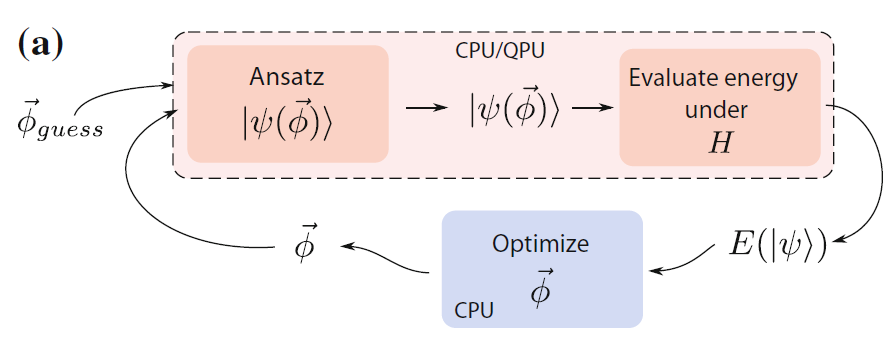
\includegraphics[scale=0.8]{VQE.PNG}
    \caption{Someone pls could draw a pic like this? This is from Shadbolt's Thesis.}
    \label{fig:VQE}
\end{figure}
%%%%%%%%%%%%

\subsubsection{Aside: Deriving inequality \autoref{eq:inequality}}
\hrule
\vspace{\baselineskip}
We have that we can write any state in terms of the energy basis $\{\ket{\lambda_i}\}$, the Ansatz in particular as:
\begin{align*}
    \ket{\psi(\theta)}=\sum^n_{i=0} \psi_i \ket{\lambda_i}, \hspace{0.5cm} \psi_i \in \mathds{C}, \hspace{0.5cm}\sum^n_{i=0} |\psi_i|^2=1.
\end{align*}
Considering the expected value for the energy of the system in that state we have:
\begin{align*}
    H\ket{\psi(\theta)}=\sum^n_{i=0} \psi_i H\ket{\lambda_i}=\sum^n_{i=0} \psi_i \lambda_i\ket{\lambda_i}.
\end{align*}
Considering the expected value for the energy in the state $\ket{\psi(\theta)}$:
\begin{align*}
    \lambda_{\psi(\theta)}=\left < \psi(\theta)|H| \psi(\theta)\right>=\sum^n_{i=0} |\psi_i|^2 \lambda_i\geq \sum^n_{i=0} |\psi_i|^2 \lambda_0= \lambda_0 \sum^n_{i=0} |\psi_i|^2 =\lambda_0.
\end{align*}
Therefore we get the inequality:
\begin{align*}
   \lambda_{\psi(\theta)}=\left <\psi(\theta)|H| \psi(\theta)\right> \geq \left< \lambda_0|H| \lambda_0\right>= \lambda_0.
\end{align*}
%proof\\
\hrule
\vspace{\baselineskip}

%%%%%%%%%%%%%%%%%%%%%%%%%%%%%%%%%%%%%%%%%%%%%%%%%%%%%%%%
\section{Summary of algorithms covered in this chapter}

\begin{center}
\begin{table}[H]
\begin{tabular}{|>{\centering\arraybackslash}m{.15\textwidth}|>{\centering\arraybackslash}m{.19\textwidth}|>{\centering\arraybackslash}m{.19\textwidth}|>{\centering\arraybackslash}m{.21\textwidth}|>{\centering\arraybackslash}m{.17\textwidth}|}
    \hline
    \textbf{Algorithm} & \textbf{Purpose} & \textbf{Number of qubits required} & \textbf{Number of gates required} & \textbf{Success probability}\\
    
    \hline
    
    Grover's algorithm & Unstructured search & $n$ qubits for $2^n$ marked elements & $(2T+1)n$ Hadamard gates,$T$ $U_f$ gates, and $T$ $U_0$ gates, where $T \approx \frac{\pi}{4} \sqrt{2^n}$ & $\sin^2((2T+1)\arcsin{\frac{1}{\sqrt{2^n}}})$\\
    \hline
    
    Quantum period finding & Finding Periodicity & & & \\
    \hline
    
    Deutsch-Jozsa algorithm & Constant or Balanced function & $n+1$ qubits for $2^n$ elements & One $U_{f}$ gate and $2n+1$ Hadamard gates & 100\% \\
    \hline
    
    Eigensolver & & & & \\
    \hline
    
    Shor's Algorithm & Factor a large number $N$ & $4\ln(N)/\ln(2) \leq n < 4\ln(2N)/\ln(2)$ & $n < 4\ln(2N)/\ln(2)$ $H$ gates, $U_f$ gate, QFT gate &\\
    \hline 
    
    \end{tabular}
\caption {Table of Quantum Algorithms} 
\end{table}
\label{AlgorithmTable} 
\end{center}


